\title{HomoLogical Algebra}
\author{
       Brian Droncheff
}

\documentclass[12pt]{report}
\usepackage{verbatim}
\usepackage{amsmath}
\usepackage{amssymb}
\usepackage{tikz-cd}
\usepackage{tikz}
\usepackage{tikz-3dplot}
\usepackage{scalerel}
\usepackage{stackengine}
\usepackage{mathrsfs}
\usepackage[all]{xy}
\usepackage{graphicx}
\usepackage{subcaption}
\usepackage{hyperref}
\usepackage{titlesec}     
\usepackage{changepage}
\usepackage{parallel,enumitem}
\usepackage[all]{xy}
\usepackage{floatrow}
\usepackage{glossaries}
\usepackage [autostyle, english = american]{csquotes}

\usetikzlibrary{calc,intersections}
\usetikzlibrary{positioning}
\usetikzlibrary{shapes.geometric,calc,through}

\newtheorem{theorem}{Theorem}[section]
\newtheorem{lemma}[theorem]{Lemma}
\newtheorem{proposition}[theorem]{Proposition}
\newtheorem{corollary}[theorem]{Corollary}
\newtheorem{example}[theorem]{Example}
\newtheorem{postulate}[theorem]{Postulate}
\newtheorem{diagram}[theorem]{Diagram}


\newenvironment{proof}[1][Proof]{\begin{trivlist}
\item[\hskip \labelsep {\bfseries #1}]}{\end{trivlist}}
\newenvironment{definition}[1][Definition]{\begin{trivlist}
\item[\hskip \labelsep {\bfseries #1}]}{\end{trivlist}}
\newenvironment{question}[1][Question]{\begin{trivlist}
\item[\hskip \labelsep {\bfseries #1}]}{\end{trivlist}}
\newenvironment{note}[1][Note]{\begin{trivlist}
\item[\hskip \labelsep {\bfseries #1}]}{\end{trivlist}}


\newcommand{\qed}{\nobreak \ifvmode \relax \else
      \ifdim\lastskip<1.5em \hskip-\lastskip
      \hskip1.5em plus0em minus0.5em \fi \nobreak
      \vrule height0.75em width0.5em depth0.25em\fi}
\newcommand{\noteend}{\nobreak \ifvmode \relax \else
      \ifdim\lastskip<1.5em \hskip-\lastskip
      \fi \nobreak
      \vrule height0.3em width0.3em depth0.25em\fi}
\newcommand{\defend}{$\spadesuit$}
\newcommand{\exend}{$\blacklozenge$}
\newcommand{\tb}{$\hspace*{.5cm}$}
\newcommand{\ltb}{$\hspace*{1cm}$}
\newcommand{\smsp}{$\hspace*{.1cm}$}
\newcommand{\smnl}{$\\[.25cm]$}
\newcommand{\dnl}{$\\[.5cm]$}
\newcommand{\Lim}[1]{\raisebox{0.5ex}{\scalebox{0.8}{$\displaystyle \lim_{#1}\;$}}}
\newcommand*{\inbk}[1]{$\langle {#1}|{#1} \rangle $}
\newcommand*{\otbk}[1]{$|{#1} \rangle \langle {#1}|$}
\newcommand*{\inbktwo}[2]{$\langle {#1}|{#2} \rangle $}
\newcommand*{\otbktwo}[2]{$|{#1} \rangle \langle {#2}|$}
\newcommand*{\otbkthree}[3]{${#1}|[#2]\rangle \langle [#2]|{#3} $}
\newcommand*{\inbkthree}[3]{$\langle {#1}|[#2]|{#3} \rangle $}
\newcommand{\rowtens}[2]{$|{#1} \rangle \otimes |{#2} \rangle$}
\newcommand{\coltens}[2]{$ \langle{#1}| \otimes  \langle{#2}|$}
\newcommand{\ket}[1]{$|{#1}\rangle$}
\newcommand{\bra}[1]{$\langle{#1}|$}
\newcommand{\tit}[1]{$\textit{#1}$}
\newcommand{\tbf}[1]{$\textbf{#1}$}
\newcommand*\circled[1]{\tikz[baseline=(char.base)]{
            \node[shape=circle,draw,inner sep=-.35pt] (char) {#1};}}
\newcommand{\ketrep}[1]{$[|{#1}\rangle]$}
\newcommand{\brarep}[1]{$[\langle{#1}|]$}
\newcommand{\ketreparg}[2]{${#1}[|\rangle]{#2}$}
\newcommand{\brareparg}[2]{${#1}[\langle|]{#2}$}
\newcommand{\comm}[2]{$ \left[{#1},{#2}\right]={#1}{#2}-{#2}{#1}$}
\newcommand{\tensormult}[4]{$\begin{bmatrix} #1#3 & #1#4 \\ #2#3 & #2#4 \end{bmatrix}$}
\newcommand{\tens}[2]{${#1} \otimes {#2}$}
          

%\def\subcap{\mathrel{\ThisStyle{\kern.7pt\stackinset{c}{-.3\LMpt}{b}{.8\LMpt}%
 % {\scalebox{1.5}[1]{$\SavedStyle\subset$}}%
 % {\scalebox{1}[1.5]{$\SavedStyle\cap$}}}\kern .3pt}}
\def\impax{\mathrel{\ThisStyle{\kern 0pt\stackinset{c}{0\LMpt}{b}{3\LMpt}%
  {\scalebox{1}[1]{$\SavedStyle\Leftrightarrow$}}%
  {\scalebox{1}[1]{$\SavedStyle\Updownarrow$}}}\kern 0pt}}
\makeatletter
\newcommand{\superimpose}[2]{%
  {\ooalign{$#1\@firstoftwo#2$\cr\hfil$#1\@secondoftwo#2$\hfil\cr}}}
\makeatother
\newcommand{\subsetintersection}{\mathpalette\superimpose{{\subset}{\cap}}}
\newenvironment{pindent}{\begin{adjustwidth}{1cm}{1cm}}{\end{adjustwidth}}

\MakeOuterQuote{"}
\begin{document}
\subsection{Exact Sequences}
\tb Exact sequences give the logical distance between logical expressions. As we will see, exact sequences are similar to 'polarizers' which are operators. \textcolor{green}{Polarization is a operation via projection operators?, after which we will apply the measurement operator to the resulting (polarized) logical expression.}
\tb Now we investigate exact sequences of logical expressions. Let $L_1, L_2 \in \mathcal{L}$ where $\mathcal{L}$ is the set of logical expressions. We build the short exact sequence: 
$$0 \rightarrow L_1 \wedge L_2 \rightarrow L_1 \vee L_2 \rightarrow (L_1 \vee L_2) / (L_1 \wedge L_2) \rightarrow 0$$
As $(L_1 \vee L_2) / (L_1 \wedge L_2) = (L_1 \vee L_2) \wedge \neg(L_1 \wedge L_2) = (L_1 \Updownarrow L_2)$ we have found two expressions that are distinguishable from one another. We have shown by the exact sequence how $L_1 \wedge L_2$ is related to $L_1 \vee L_2$ in that it is related via the XOR operator. \smnl
Hence $\partial: L_1 \wedge L_2 \rightarrow L_1 \Updownarrow L_2$. Note that this is projection is equivalent to $$(L_1 \vee L_2) \wedge \neg(L_1 \wedge L_2) = L_1 \Updownarrow L_2$$ 
Which we can model by an exact sequence:
$$0 \overset{\alpha}{\longrightarrow} [\wedge] \overset{\beta}{\longrightarrow}  [\vee] \overset{\gamma}{\longrightarrow} [\vee]/[\wedge] \overset{\delta}{\longrightarrow} 0$$
where $[\wedge]/[\vee] = [\Updownarrow]$. For this chain to be exact we have to have that $im(\alpha) = ker (\beta)$, $im(\beta) = ker(\gamma)$, and $im(\gamma) = ker(\delta)$. We can see that the above sequence is exact as $\alpha$ is the $0$-map and $\beta$ is injective, $im(\beta) = ker(\gamma)$ as by construction $ker(\gamma) = [\vee]/[\wedge]$, and $im(\gamma) = [\Updownarrow] = ker(\delta)$.   \textcolor{green}{need to define $0$-map and injective in terms of logical matrices}. We have a homology as $im(\beta) / ker(\gamma) = \{\emptyset\}$.


We first look at the relationship between two logical exact sequences via the logical expressions as partitioned sets

\[
\begin{tikzcd}
0 \ar{r} & X \wedge \neg Y \ar{r}{\vee (X \Leftrightarrow Y)} \ar{d}{(\wedge X \wedge Y \wedge \neg Z) \vee X \wedge Y \wedge Z} & Y \Rightarrow X \ar{r}{\wedge (X \Leftrightarrow Y)} \ar{d}{\wedge X \vee (\neg Y \wedge Z) \vee Y \wedge Z \wedge \neg X} & X \Leftrightarrow Y \ar{r} \ar{d}{\cap \{C,D\}\cup \{A,F\}} & 0  \\
0 \ar{r} & X \Leftrightarrow Z \ar{r}{\vee X \Updownarrow Z} & X \vee Z \ar{r}{\wedge X \Updownarrow Z} & X \Updownarrow Z \ar{r} & 0
\end{tikzcd}
\]
\smnl
\[
\begin{tikzcd}
0 \ar{r} & \{A,E\} \ar{r}{\cup \{C,D,G,H\}} \ar{d}{\cap \{E\} \cup \{G\}} & \{A,C,D,E,G,H \} \ar{r}{\cap \{C,D,G,H \}} \ar{d}{\cap \{A,C,D,E,G \} \cup \{F\}} & \{C,D,G,H\} \ar{r} \ar{d}{\cap \{C,D\}\cup \{A,F\}} & 0  \\
0 \ar{r} & \{E,G\} \ar{r}{\cup \{A,C,D,F\}} & \{A,C,D,E,F,G\} \ar{r}{\cap\{A,C,D,F\}} & \{A,C,D,F\} \ar{r} & 0
\end{tikzcd}
\]
where for example $\varsigma(X \wedge \neg Y) = \{A,E\}$, $\varsigma(X \wedge Z \wedge \neg Y) = \{E\}$, $\varsigma(X \wedge Z \wedge Y)= \{G\}$, and $\varsigma(X \wedge Y) = \{E,G\}$ and going from $X \wedge \neg Y$ to $X \wedge Z$, we have the transition $((X \wedge \neg Y) \wedge (X \wedge Z \wedge \neg Y)) \vee (X \wedge Y \wedge Z) = X \wedge Y$ which corresponds to $(\{A,E\} \cap \{E\}) \cup \{G\} = \{E,G\}$. This is the methodology to get from $\{A,E\}$ to $\{E,G\}$ and corresponds to going from $X \wedge \neg Y$ to $X \wedge Y$. \smnl
\tb We can see, for example in the the second square, that we have a \textcolor{green}{homotopy (arriving at the same conclusion?}. Starting at $\{A,C,D,E,G,H\}$ and moving clockwise;
$$((\{A,C,D,E,G,H\} \cap \{C,D,G,H \}) \cap \{C,D\}) \cup \{A,F\} = \{A,C,D,F\}$$
which is equal to the clockwise movement:
$$((\{A,C,D,E,G,H\} \cap \{A,C,D,E,G\}) \cup F) \cap \{A,C,D,F \}= \{A,C,D,F \}$$
We can see by inspection that each set of transitions is exact thus we have an example of a \textcolor{green}{homology} between logical expressions!
Note that we make the identification of $\wedge$ with $\cap$ and $\vee$ with $\cup$, and furthermore that the morphisms between logical expressions in each exact rows are simply the intersection and the union of the the particular logical set! \smnl

\label{Extension (Def.)}
\begin{definition} \emph{(Extension)} \smnl
\tb Let $N$ and $Q$ be two $R-modlues$. An $R-module$ $E$ is an $\textit{extension}$ of $Q$ by $N$ if it is in an exact sequence of $R-modules$ where:

$$0 \overset{\alpha}\rightarrow N \overset{\beta}\rightarrow E \overset{\gamma}\rightarrow Q \overset{\delta}\rightarrow 0$$
\end{definition}

\[
\begin{tikzcd}
0 \ar{r} & N \ar{r}{i_1} \ar{d}{\alpha} & E_1 \ar{r}{\pi_1} \ar{d}{\eta} & Q \ar{r} \ar{d}{\gamma} &0 \\
0 \ar{r} & N \ar{r}{i_2} & E_2 \ar{r}{\pi_2} & Q \ar{r} & 0
\end{tikzcd}
\]

We let all the morphisms $f$ (i.e. $\alpha,\beta$ etc.) acting on any set $S$, by acting element wise and for $x \in S$ if $x \in im(f)$ then $f(x) = x$ and $0$ otherwise.

\[
\begin{tikzcd}[column sep=small]
0 \arrow{r} & \{B,C,D,F\} \ar{r}{i_1} \ar{d}{\alpha} & \{B,C,D,E,F,H,O,N \} \ar{r}{\pi_1} \ar{d}{\eta} & \{E,H,O,N\} \ar{r} \ar{d}{\beta} &0 \\
0 \ar{r} & \{A,B,D,M\}  \ar{r}{i_2} & \{A,B,D,E,H,M,N,O\}  \ar{r}{\pi_2} & \{E,H,O,N\}\ar{r} & 0
\end{tikzcd}
\]
Note: given the linear relationship on sets $f(x) = x$ we have that, for example: 
$$ \{A,B,D,E,H,M,N,O\} = \{A,B,D,M\} \oplus \{E,H,O,N\}$$

%\end{example}
\subsection{Continuity}
\subsubsection{Continuity}
Now we look at continuity to try and see whether one logical expression can be transformed in to another continuously and topological equivalence! Now a function $f: X \rightarrow Y$ is continuous relative to $\mathcal{T}$ and $\mathcal{T}^*$ - or is $\mathcal{T}-\mathcal{T}^*$  continuous iff $f^{- 1}(H)$ of every $\mathcal{T}^*$-open subset $H$ of $Y$ is a $\mathcal{T}$-open subset of $X$, that is iff $H \in \mathcal{T}^* \Rightarrow f^{-1}(H) \in \mathcal{T}$ and we can write $f:(X,\mathcal{T}) \rightarrow (Y,\mathcal{T}^*)$. First thing to notice is the $\Rightarrow$ in $H \in \mathcal{T}^* \Rightarrow f^{-1}(H)$. Say we explicitly let $X$ and $Y$ by logical variables then $\varsigma(X) = \{\{A\},\{B\}\}$ and  $\varsigma(X) = \{\{B\},\{C\}\}$ then $\mathcal{D}_X =  \{\{A\},\{B\}, \{A,B\}, \emptyset \}$ and  $\mathcal{D}_Y = \{\{B\},\{C\}, \{B,C\}, \emptyset \}$. Now there are several ways that we could make a map $f$ that would be continuous. Lets try to embed both of these spaces in 3 points and let $\mathcal{T}_V =  \{\{F\},\{G\}, \{F,G \}, \{F,G,H\} \emptyset \}$ and $\mathcal{T}_U =  \{\{A\},\{B\}, \{A,B\}, \{A,B,C\} \emptyset \}$. The reason for the representation is that we now have $\mathcal{D}_X \subset \mathcal{T}_U$ and $\mathcal{D}_Y \subset \mathcal{T}_V$ where $Y = G \vee H$ Now note that we have the representation for the logical variables $X$ and $Y$ that $A \rightarrow F$, $B \rightarrow G$, $C \rightarrow H$.... work out open and closed for continuous morphisms. It might be possible that the only continuous functions are those in which the image of mapping function $f$ is a subset of the pre-image and that the set of posibive truth valuations in teh image has to be a subset of positive truth valuations in the pre-image! (Verify). \smnl
Furthermore (Pg 89 in Schuams) we can find "Local Bases" of points in a topological space; let $p$ be any arbitrary point in a topological space $X$. Let $\mathcal{B}_p$ be a class of open sets containing $p$ where $\mathcal{B}_p$ is called a "local base" at $p$ iff for each open set $G$ containing $p, \exists G_p \in \mathcal{B}_p$ with the property $p \in G_p \subset G$. So considering $\mathcal{D}_{X \Rightarrow Y}$ could we say that wlog, for points $A \in S$ that $\mathcal{B}_A$ is a local base? Let $\mathcal{B}_p = \{\{A\}\}$? Now the sets $G$ that are in $\mathcal{D}_{X \Rightarrow Y}$ containing $p = A$ are $\{S, \{A,B\},\{A,C\},\{A\}\}$. We could say that for $\mathcal{B}_A = \{\{A\}\}$, that as $\forall G_A \in \mathcal{B}_A$ that $A \in G_A \subset G$. However if I tried to say that $\mathcal{B}_A = \{\{A,B\}\}$ there is an open set $G = \{A,C\}$ but $\not\exists A \in G_A \subset G$ where $G_A - \{A,B\}$!...? Note number 4 on Pg. 91. A good proof for the relations of different bases vs. different Topologies is number 6; Let $\mathcal{B}$ and $\mathcal{B}^*$ be a basis for the respective Topologies $\mathcal{T}$ and $\mathcal{T}^*$ on a set $X$ and suppose that each $B \in \mathcal{B}$ is the union of members $G^*$ in $\mathcal{B}^*$. We can show that $\mathcal{T}$ is coarser than $\mathcal{T}^*$ i.e. $\mathcal{T} \subset \mathcal{T}^*$. number 12 shows that a discrete topology can have a sub-base which does NOT include singleton sets! So if we had $\mathcal{D}_{X \Rightarrow Y}$ we could have the sub-base $\mathcal{B} = \{\{B,C\},\{B,D\},\{C,D\}\}$ as $\{B\} = \{\{B,C\} \cap \{B,D\}\}$ etc. when we transform back i.e. $\eta^{-1}(B) = \{Y, X \Leftrightarrow Y, \neg X\}$. Now note that $\{B,C\} \cap \{B,D\} \sim Y \wedge (X \Leftrightarrow Y) = X \wedge Y = B$ in partitioned logic. We also have that $\{B,C\} \cap \{C,D\} \sim Y \wedge \neg X = C$  $\{B,D\} \cap \{C,D\} = X \Leftrightarrow Y \wedge \neg X = \neg X \neg Y = D$. So indeed we can generate those singleton sets in the Topology - hence we can find the subbase or elements which build a more complex set of logical expressions!! \smnl
\tb Now looking at continuous spaces. A function $f: X \rightarrow Y$ is continuous iff the inverse of each member of a base $\mathcal{B}$ for $Y$ is an open subset of $X$. To show that the identity function $\mathcal{i}:(\mathcal{T},X) \rightarrow (\mathcal{T}^*,X)$ is continuous iff $\mathcal{T}$ is finer than $\mathcal{T}^*$ i.e. $\mathcal{T}^* \subset \mathcal{T}$. Now looking in to the coarseness of Topologies a Topology $\mathcal{T}_1$ is finer than $\mathcal{T}_2$ if every open set in $\mathcal{T}_2$ is open in $\mathcal{T}_1$ i.e. $\mathcal{T}_2 \subset \mathcal{T}_1$ we can also say that $\mathcal{T}_2$ is more coarse than $\mathcal{T}_1$. \smnl
\tb So taking $\mathcal{D}_Y = \{B\},\{C\},\{B,C\}, \emptyset \}$ and $\mathcal{D}_{X \Rightarrow Y}$ that $\mathcal{D}_X \subset \mathcal{D}_{X \Rightarrow Y}$ hence $\mathcal{D}_{X \Rightarrow Y}$ is finer than $\mathcal{D}_Y$ this means that if we use the identity function $\mathcal{i}$ we would however have to have the same set $X$ as to which $\mathcal{i}$ maps i.e. $\mathcal{i}:(\mathcal{T},S) \rightarrow (\mathcal{T}^*, S)$ so both the $D_{X \Rightarrow Y}$ and $\mathcal{D}_{Y}$ embedded in the space $S = \{A,B,C,D \}$ So we would have $\mathcal{i}:(\mathcal{T}_{X \Rightarrow Y},S) \rightarrow (\mathcal{T}_Y, S)$ in which for each $G \in \mathcal{T}_Y$ as $\mathcal{i}^{-1}(G) \in \mathcal{T}_{X \Rightarrow Y}$ we have that $\mathcal{i}$ is continuous and also we demonstrate that we can find a continuous function from the set of positive valuations of a logical expression with a restriction on its positive valuations (a subset of positive valuations). \smnl

\subsection{Pushouts}
\tb Here we check out pushouts.
\begin{center}

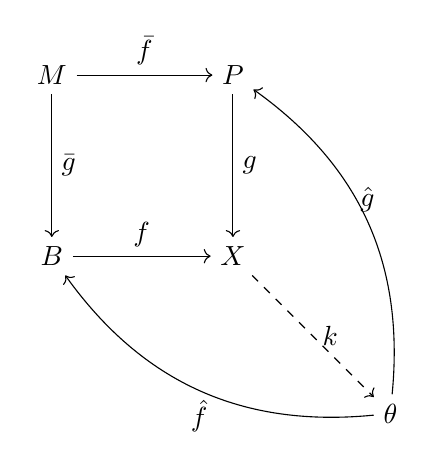
\begin{tikzpicture}
  \node (P) {$M$};
  \node (B) [node distance=2.3cm, right of=P] {$P$};
  \node (A) [node distance=2.3cm, below of=P] {$B$};
  \node (C) [node distance=2.3cm, below of=B] {$X$};
  \node (P1) [node distance=2cm, right of=C, below of=C] {$\theta$};
  \draw[->] (P) to node [above] {$\bar{f}$} (B);
  \draw[->] (P) to node  [right] {$\bar{g}$} (A);
  \draw[->] (A) to node [above] {$f$} (C);
  \draw[->] (B) to node [right] {$g$} (C);
  \draw[->, bend right] (P1) to node [above] {$\hat{g}$} (B);
  \draw[->, bend left] (P1) to node [below] {$\hat{f}$} (A);
  \draw[->, dashed] (C) to node [right] {$k$} (P1);
\end{tikzpicture}
\end{center}
\begin{theorem}
\tb If we have a commutative diagram:
\[
\begin{tikzcd}
0 \ar{r} & M \ar{r}{i} \ar{d}{\beta} & P \ar{r}{\sigma} \ar{d}{\alpha} & A \ar{r} \ar{d}{id} &0 \\
0 \ar{r} & B \ar{r}{j} & X \ar{r}{\tau} & A \ar{r} & 0
\end{tikzcd}
\]
Then $X$ is the pushout of $B$ and $P$ with respect to $i$ and $\beta$. For the proof see $\href{https://www.math.nmsu.edu/~pmorandi/math683f00/PushoutsPullbacks.pdf}{\text{"here"}}$ \smnl
\end{theorem}
\begin{question} a) Check that the morphism of extensions is always an isomorphism. \smnl
\tb When two extensions are equivalent (congruent) such as they are in the below diagram, then there is a group isomorphism $\alpha: G \rightarrow G$ which makes the diagram commute.\smnl
\tb If we have a commutative diagram:
\[
\begin{tikzcd}
0 \ar{r} & N \ar{r}{i_1} \ar{d}{id} & E_1 \ar{r}{\pi} \ar{d}{\alpha} & Q \ar{r} \ar{d}{id} &0 \\
0 \ar{r} & N \ar{r}{i'} & E_2 \ar{r}{\pi '} & Q \ar{r} & 0
\end{tikzcd}
\]
\tb $\alpha$ however is always an isomorphism when sandwiched between the $id$ maps between the exact sequences above. This is due two the $\href{https://en.wikipedia.org/wiki/Five_lemma}{\text{"Five Lemma"}}$, and more specifically the $\href{https://en.wikipedia.org/wiki/Short_five_lemma}{\text{"Short Five Lemma"}}$. Proof of the Five Lemma is in the linked page, and linked is $\href{http://everything2.com/title/short+five+lemma}{\text{"Short Five Lemma Proof"}}$.
\end{question}

\tb Let $E = N \cup Q$ $\forall s \in \sigma Q, i^{-1}(s) \not\in N$ by exactness hence there is no $n \in N$ such that $i(n) = \pi(x)$ for $x \in E$ other than the identity. Thus as $\pi(x) = \sigma(s)$ we have that $i(N) \cap \pi(Q) = e \Rightarrow i(n) \cap \sigma(s) = e \therefore i(N) \cap \sigma(Q) = e$ Now by exactness as we have $0$ coming in and going out we have to have that $E = N \oplus Q$. \smnl
\tb Proof of the splitting lemma is here: $\href{https://en.wikipedia.org/wiki/Splitting_lemma}{\text{"Splitting Lemma"}}$. Now, according to the splitting lemma, if the exact sequence admits a morphism $i':E \rightarrow N$ such that $i' \circ i = id_N$ or $\pi':E \rightarrow Q$ such that $\pi' \circ \pi = id_Q$ then $E$ is a twisted direct sum of $N$ and $Q$.
\smnl
\[
\begin{tikzcd}
0 \ar{r} & N \ar{r}{i}  & E \ar{r}{\pi} \ar{l}{j} & Q \ar{r} \ar{l}{\sigma}  &0 \\
\end{tikzcd}
\]
where $j \circ i(N) = id_N$ \smnl
\tb We start by showing that each element $e$ is in $\{im(i) + ker(j)\}$. The reason for this is that, by exactness we know that $ker(j) = im(\sigma)$ and thus every element in $E$ maps to some element in $N$ or is mapped from some element in $P$. We know that $e= e - i \circ j(e) +i \circ j(e) \forall e \in E$ and that $i \circ j(e) \in E$. Now for the remaining terms; $j(e) = j(e) - j \circ i \circ j(e)$ by homomorphism over the mapping $j$ and we are left with $j(e) - j(e) = 0$ as again $j \circ i(N) = id_N$ and so $j\circ i \circ j (e) = (j\circ i) \circ j (e) = j(e)$. We then have that if $e \not\in \, im(i)$ then it must be that $j(e) - j(e) = 0$ hence $e \in ker (j)$. But we also want to show that $0 \neq e \not\in im(i) \cap ker(j)$. Say it is, then as  $i(n) = e$ for some $n \in N$ and $j(e) = 0$ we have that $j(i(n)) = 0$ so by the restriction that $j(i(n)) = n$ we have that $n = 0$. Thus $e \in im(i) \oplus ker(j) \forall e \in E$. \smnl

 Now we want to show isomorphisms for exactness. We know that $im(i) \oplus ker(j)$ and also that $e \in E$ where $e = e - j \circ i(n) + i \circ j(n) $ but that $i \circ j(n) \in im(i)$ and $e = e - j \circ i(n)$ so $j(e) = j(e) - j \circ i \circ j(e) = 0$ and so $e \in ker(j)$ thus all $e$ are accounted for. We then know every element $e$, as it is in the image of $i$ or kernel of $j$ that $e = i(a)$ or $e \in ker (j)$ so $e = i(a) + k$ where $k \in ker(j)$. Now by exactness we know that $\forall p \in P \exists e \in E$ such that $\pi (e) = p$, but as $e$ can be associated with some unique element $i(a)+ k$ we have that $\pi (i(a) + k) = p$, but as $im(i) = ker(\pi)$ we have that $\pi$ we have $\pi (i(a)) = 0$ so $\pi (k) = p$. The key however is that as $\pi$ is surjective, that $\forall p \exists k$ such that $\pi (k) = p$. So $\pi \circ ker(j) = p$. Now if $\pi (k) = 0$ then $k \in im(i)$, but as $k \in im(j)$ as well we have to have that $k \in (im(i) + ker (j))$ so $k = 0$. This means that there are just enough $k$'s $\neq 0$ such that $\pi (k) = p$. Thus we have to have that the restriction of $\pi : ker(j) \rightarrow p$ is an isomorphism, so $ker(j) \simeq p$. Now as $im(i)$ is injective, $im(i) \simeq N$ so as $ker(j) \simeq p$ and $im(i) \simeq p$ and $E \simeq im(i) \oplus ker(j)$ then $E \simeq N \oplus Q$.

Then $X$ is the pushout of $B$ and $P$ with respect to $i$ and $\beta$. For the proof see $\href{https://www.math.nmsu.edu/~pmorandi/math683f00/PushoutsPullbacks.pdf}{\text{"here"}}$ \smnl
\tb There is also proofs of the extensions of the pullbacks and pushouts $\href{http://sierra.nmsu.edu/morandi/oldwebpages/math683fall2002/Ext.pdf}{here}$

We want to show that the pushout:

\begin{center}

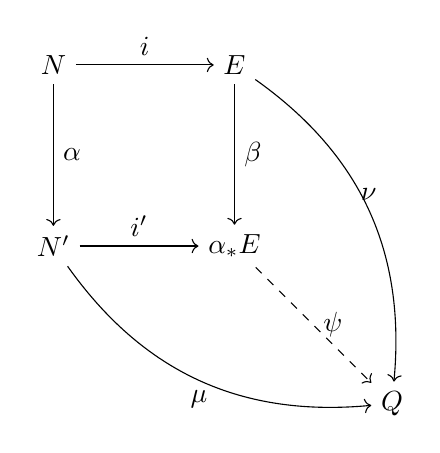
\begin{tikzpicture}
  \node (P) {$N$};
  \node (B) [node distance=2.3cm, right of=P] {$E$};
  \node (A) [node distance=2.3cm, below of=P] {$N'$};
  \node (C) [node distance=2.3cm, below of=B] {$\alpha_{*}E$};
  \node (P1) [node distance=2cm, right of=C, below of=C] {$Q$};
  \draw[->] (P) to node [above] {$i$} (B);
  \draw[->] (P) to node  [right] {$\alpha$} (A);
  \draw[->] (A) to node [above] {$i'$} (C);
  \draw[->] (B) to node [right] {$\beta$} (C);
  \draw[->, bend left] (B) to node [above] {$\nu$} (P1);
  \draw[->, bend right] (A) to node [below] {$\mu $} (P1);
  \draw[->, dashed] (C) to node [right] {$\psi$} (P1);
\end{tikzpicture}
\end{center}


Consider the commutative diagram:

\[
\begin{tikzcd}
0 \ar{r} & N \ar{r}{i} \ar{d}{\alpha} & E \ar{r}{\pi} \ar{d}{\beta} & Q \ar{r} \ar{d}{id} &0 \\
0 \ar{r} & N' \ar{r}{i'} & \alpha_{*}E \ar{r}{\pi '} & Q \ar{r} & 0
\end{tikzcd}
\]
\tb To show that  $\psi$ is unique. Let  $\psi$ be a map and that  $\psi(i'(N') + \beta (E)) = (\nu(N') + \mu (E)$. Now say there is another map $\phi$ such that $\phi(i'(N') + \beta (E)) = \phi(i'(N')) + \phi(\beta (E)) = \nu(N') + \mu (E)$ then $\phi = \psi$. \smnl
\tb To show that $\psi$ is well defined we need to show that if $\psi (i'(N') + \beta (E)) = 0$ that $ \nu(N') + \mu (E) = 0$. Now let $y \in E$ and that $\beta (y) + i'(n') = 0$. Applying $\pi '$ we get $\pi '(\beta (y) + i'(n')) = \pi '(\beta(y)) + \pi '(i'(n'))$ via homomorphism and that $\pi '(i'(n')) = 0$ by exactness. Thus we have that $\pi '(\beta(y)) = 0$. We however have that $\pi '(\beta(y)) = \pi(y) = 0 \therefore y \in ker(\pi)$ hence we have that $n \in N$ such that $i(n) = y$. \smnl
\tb Rewriting the original expression we have that $\beta (y) + i'(n') = \beta(i(n))+i'(n') = 0$. Now $\beta(i(n)) = i'(\alpha (n))$ so we have that $ i'(\alpha (n)) + i'(n') = 0$, hence as $i'$ is injective, by the homomorphism property we know that $i'(\alpha(n) + n')=0$ and so $\alpha(n) + n' \Rightarrow \alpha(n) = n'$. Knowing this we have $\nu(n') + \mu (y)$ in which we know that $i(n) = y$ and $n' = \alpha (n)$ which gives $\nu(- \alpha (n)) + \mu (i(n))$. Now as $\nu \circ \alpha = \mu  \circ i$ by commutativity, we have that as $-g = -i' ( \alpha(n))$ and $g = \mu (i(n))$ that $\nu(- \alpha (n)) + \mu (i(n)) = -g + g = 0$! So we have proved that $\psi (i'(n)) + \beta (y)) = 0 \Rightarrow \nu (n') + \mu  (y) = 0$. \smnl
\tb Now as $\pi$ is surjective by exactness and, that $\pi(E) = \pi ' \circ \beta (E)$ by commutativity, we have that $\pi '$ is surjective. We also know that $\pi ' \circ i ' = 0$ by definition of a pushout ($\alpha_{*}E$ is universal) and we want to show that $im(i') = ker(\pi ')$ and that $i'$ is injective. We do this by the definition of $\alpha_{*}E = N' \oplus E/S$ where $S = (\alpha(n),-i(n)), n \in N$. Now letting $i'$ be defined by $i'(n') = (n',0) + S$ and $\beta(e) = (0,e) + S$. Also that $\pi '$ is defined by $\pi '((n',e) + S) = \pi (e)$ ($S$ and $n'$ are in $ker(\pi ')$, the latter by exactness). So we have that $ker(\pi ') = \{(n',e) + S: \pi(e) = 0 \}$ which means that $e \in ker(\pi) \therefore e \in im(i)$. As $e \in im(i)$ we let $e = i(n): n \in N$ thus we have the set $\{(n',i(n)):n \in N, n' \in N' \} = \{(n' + \alpha(n),0)+S) \} = i'(N')$. So we have that $ker(\pi ') = im(i')$. Last we have that $ker(i') = \{n' \in N':(n',0) \in S \}$. If $(n',0) \in S$, then there is an $n \in N$ with $(n',0) = (\alpha(n),-i(n))$ in which we can conclude that $i(n) = 0 \Rightarrow n = 0$. We have then that $n' = \alpha(0) = 0$ and we then have left arrow from zero in to $N'$ and that $\alpha_{*}E$ is an extension of $Q$ by $N'$. \smnl
\end{document}
